% Session 6 -- what a magnon is in real space, and the Holstein-Primakoff bookkeeping.
% Placement: sec. "The Holstein-Primakoff transformation", at the paragraph that states the
% bookkeeping (S^- creates a magnon, S^+ destroys one) after eq. (6.7).
% Rendered by figures/blender/s06f05_magnon.py, labels in figures/overlays/s06f05_magnon.tex.
\begin{aqmfigure}{fig:s06:magnon}{The states that (6.6) and (6.7) describe. (a) The ferromagnetic
ground state, where every spin has its maximal value $S^z=S$, and so there are no magnons. (b) A
single magnon is \emph{not} one spin flipped on one site. Instead, every spin is tilted slightly out
of alignment and precesses on its cone, and the precession phase advances by $\mathbf
k\cdot\boldsymbol\delta$ from one site to the next. This is seen most clearly in the view from
above, where the transverse component turns at a constant rate and comes back to itself after one
wavelength. The missing unit of spin is therefore shared coherently by the whole lattice, and
$\sum_i\langle S_i^z\rangle=NS-1$. Since the tilting angle is small, we have $\langle a_i^\dagger
a_i\rangle\ll S$ everywhere, which is the condition under which we can expand the square roots in
(6.6). In the drawing the tilting angle is much larger than in reality. (c) The counting rule that
makes the transformation easy to remember. The boson number counts the spin removed from saturation,
so the \emph{lowering} operator $S^-$ creates a magnon and the \emph{raising} operator $S^+$
destroys one.}
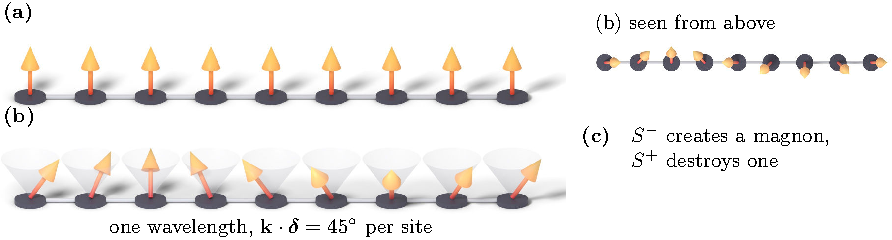
\includegraphics{figures/pdf/s06f05_magnon.pdf}
\end{aqmfigure}
